\documentclass[10pt,a4paper]{article}
\usepackage[utf8]{inputenc}
\usepackage{amsmath}
\usepackage{amsfonts}
\usepackage{amssymb}
\usepackage{graphicx}
\usepackage{caption}
\usepackage{subcaption}

\author{Daniel Brown and Dohyun Kim}
\title{Exploration of Different Gradient Descent Methods for Bayesian Inverse Reinforcement Learning}
\begin{document}
\maketitle

\section{Introduction}
Markov Decision Processes (MDPs) are a commonly used model for sequential decision making tasks. Many different methods including as dynamic programming and temporal difference methods have been proposed to allow a learning agent to solve for the optimal policy of an MDP. However, in some tasks it can be hard to specify a reward function and may be easier to provide demonstrations. This leads to the problem of Inverse Reinforcement Learning (IRL) \cite{ng2000algorithms}. Given an MDP$\setminus$R (an MDP without a specified reward function), and a set of demonstrations consisting of state-action pairs, we wish to recover the reward function that makes the demonstrations optimal. 

Many approaches have been proposed to solve this problem. We choose to focus on the Bayesian IRL setting \cite{ramachandran2007bayesian}. Gradient methods have been proposed to solve this problem \cite{lopes2009active,choi2011map} but contain no details about the specifics of how to perform gradient descent. We seek to find the MAP estimate of the true reward by maximizing the posterior of the reward $R$ given a set of demonstrations $D$ where
\begin{equation}
P(R | D) \propto P(D | R) P(R)
\end{equation}
The likelihood $P(D|R)$ is defined in a form of softmax function \cite{sutton1998reinforcement} as 
\begin{equation}
P(D | R) = \frac{e^{\alpha \sum_i Q^*(s_i,a_i;R)}}{\sum_{b \in A} e^{\alpha \sum_i Q^*(s_i,b;R)}}
\end{equation}
where $Q^*(s,a; R)$ is the optimal Q-value function for reward $R$ and $\alpha$ is a confidence parameter defining how reliable the demonstrations are. The prior $P(R)$ can be any function. 

We want to use gradient ascent to update to find 
\begin{equation}
R_{MAP} = \arg \max_R  P(R | D) = \arg \max_R [\log(P(D|R) + \log P(R)]
\end{equation}
 reward function to maximize the posterior, thus our update takes the form
\begin{equation}
R_{new} \leftarrow R + \eta_t \nabla_R [\log(P(D|R) + \log P(R)]
\end{equation}

We propose to explore some of the different flavors of gradient descent we have discussed in class as they apply to the problem of solving the IRL problem.

\section{Gradient Computation}
We first considered just the maximum likelihood estimate of the reward (corresponding to a uniform prior). To perform gradient descent we need to find the gradient of the likelihood function. We have 
\begin{eqnarray}
\nabla_R \log P(D | R) = \nabla_R \log \prod_{(s,a) \in D} P(a | s, R) \\
=\sum_{(s,a) \in D} \nabla_R \log \frac{e^{\alpha Q_R^*(s,a)}}{\sum_{b \in A} e^{\alpha Q_R^*(s,b)}}\\
= \sum_{(s,a) \in D} \nabla_R \alpha Q_R^*(s,a) - \log \sum_{b \in A} e^{\alpha Q_R^*(s,b)}\\
= \sum_{(s,a) \in D} \alpha \nabla_R Q_R^*(s,a) - \frac{\alpha}{Z_a}\bigg(\sum_{b \in A} e^{\alpha Q_R^*(s,b)} \nabla_R Q_R^*(s,b)\bigg)\\
\end{eqnarray}

where 
\begin{equation}
Z_a = \sum_{b \in A} e^{\alpha Q_R^*(s,b)}
\end{equation}
To compute $\nabla_R Q^*_R(s,u)$ for some action $u$, we note that 
\begin{equation}
V^{\pi} = R + \gamma T^{\pi} V^{\pi}
\end{equation}
so 
\begin{equation}
Q^*_u = R + \gamma T^a V^{\pi^*} = R + \gamma T^a(I - \gamma T^{\pi^*})^{-1}R
\end{equation}
and
\begin{eqnarray}
\frac{\partial Q(s,u)}{\partial R_i} = \delta_i(s) + \gamma W(s,i)
\end{eqnarray}
where $W = T^a(I - \gamma T^{\pi^*})^{-1}$

\section{Approach}
We propose to investigate a simple, yet scalable navigation domain where a subset of states have negative reward (obstacles) most states have zero reward and the goal state has positive reward. Given a few demonstration trajectories, we wish to recover the reward using gradient descent.

We propose to investigate the following gradient descent methods: standard gradient descent (GD) with full step size, GD with BTLS, and accelerated GD.

We also hope to also investigate whether using a sparsity-inducing l1 regularization term can help find a sparse reward function that matches the demonstrator's reward. We will compare the Frank-Wolfe, and subgradient descent methods to maximize the likelihood minus the regularization. 

\section{Results}
\subsection{Recovering a sparse reward}
We noticed that even though gradient ascent usually recovers the optimal policy, the reward it finds is rarely sparse. However, in many sequential decision making tasks the reward is sparse. To try to better recover the expert's true reward when the reward is known to be sparse we added an $L^1$-norm regularization. Our new objective function is 
\begin{equation}
\max_R \log P(D|R) - \lambda \|R\|_1
\end{equation}

To test this method out we designed a simple $4\times 7$ grid navigation task where there is a winding path of smooth ground where travel costs are zero and patches of rough ground where travel costs are -1, there is also a terminal goal state with a reward of +1 in the top left corner. The true reward is shown in Figure~\ref{subfig:true_sparse_reward}. We optimized the regularized objective using subgradient descent for different values of the regularization parameter $\lambda$.

\begin{figure}
    \centering
    \begin{subfigure}[b]{0.45\textwidth}
        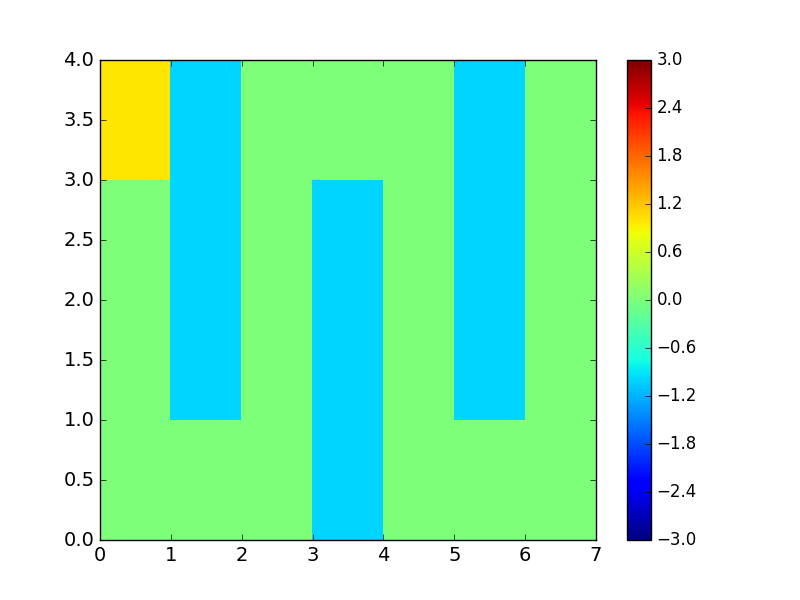
\includegraphics[width=\textwidth]{figs/true_reward.png}
        \caption{True sparse reward used by demonstrator}
        \label{subfig:true_sparse_reward}
    \end{subfigure}
    ~ %add desired spacing between images, e. g. ~, \quad, \qquad, \hfill etc. 
      %(or a blank line to force the subfigure onto a new line)
    \begin{subfigure}[b]{0.45\textwidth}
        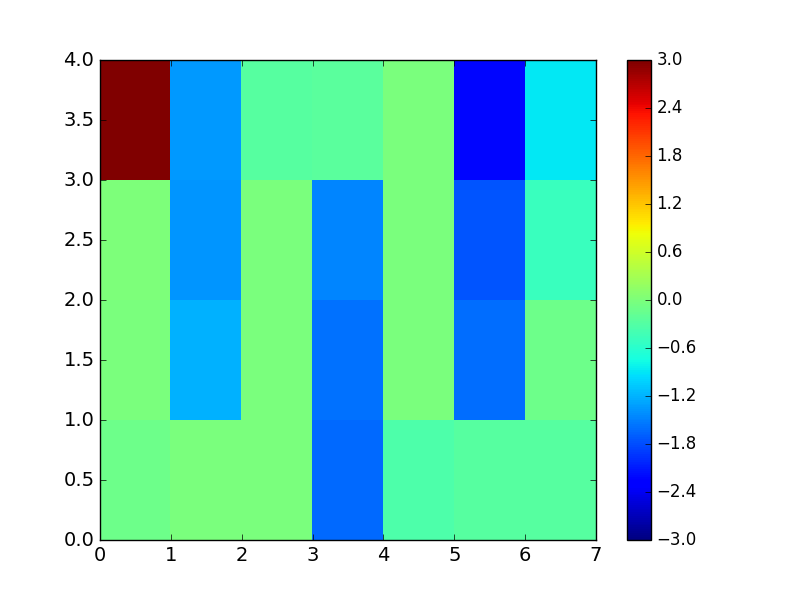
\includegraphics[width=\textwidth]{figs/recovered_reward_lam0_5.png}
        \caption{Recovered reward using regularization with $\lambda = 0.5$}
        \label{subfig:recovered_sparse_reward}
    \end{subfigure}
    \caption{True and recovered sparse reward. Sparse reward is learned using subgradient descent.}\label{fig:sparse_reward}
\end{figure}

Figure~\ref{fig:regularization_test} shows the results. We see if Figure~\ref{subfig:reg_L1-norm} that, as expected, higher regularization results in lower $L^1$-norm of the learned reward. We also see in Figure~\ref{subfig:reg_reward_diff} that using a larger regularization term results in a recovered reward that is much closer to that of the experts. Figure~\ref{subfig:reg_policy_diff} shows that too much regularization ($\lambda = 1.0$) causes the algorithm to find a sparse reward that does not result in a good policy, while a regularization term of $\lambda = 0.5$ seems to do best in terms of recovering a sparse reward that still induces a policy that matches the expert. We have plotted a heatmap of the learned reward when $\lambda=0.5$ in Figure~\ref{subfig:recovered_sparse_reward}. The regularization helps the algorithm to find a reward that is close to zero along the path and has non-zero rewards at the goal and along the rougher terrain.

 Interestingly, the tests run with smaller regularization terms immediately found rewards that produced the expert's policy, which is why the lines are not visible in Figure~\ref{subfig:reg_policy_diff}; however, using these smaller regularization terms resulted in a type of reward overfitting, where non-sparse rewards were learned to try to maximize the likelihood of the demonstrations.


\begin{figure}
    \centering
    \begin{subfigure}[b]{0.65\textwidth}
        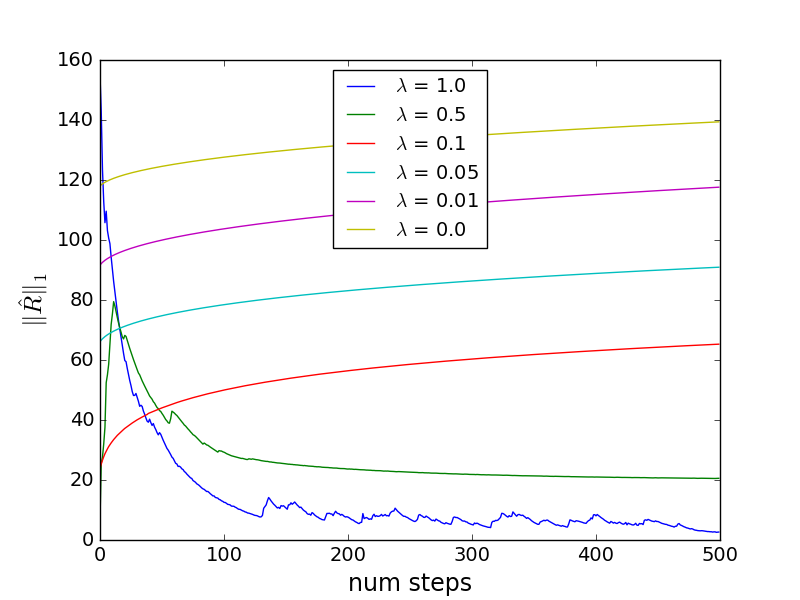
\includegraphics[width=\textwidth]{figs/reward_norm_reg_test.png}
        \caption{$L^1$-norm of learned reward function.}
        \label{subfig:reg_L1-norm}
    \end{subfigure}
    \begin{subfigure}[b]{0.65\textwidth}
        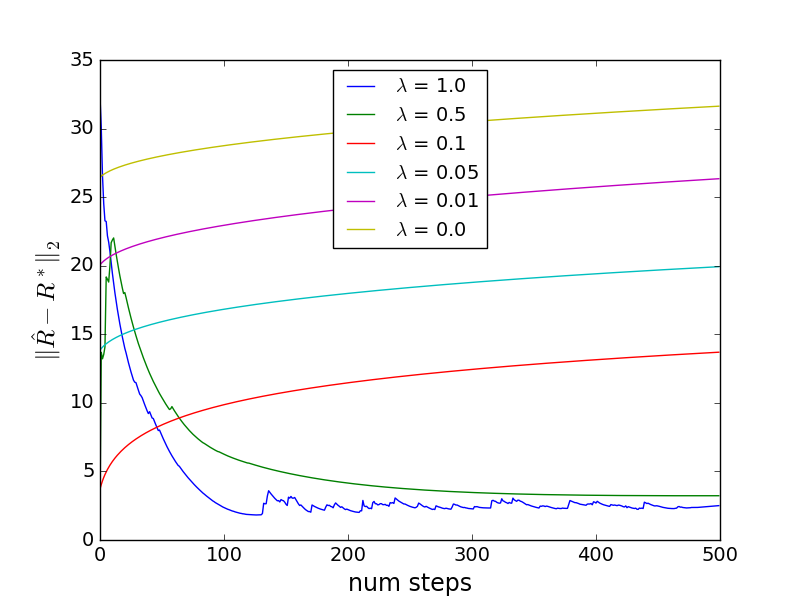
\includegraphics[width=\textwidth]{figs/reward_diff_reg_test.png}
        \caption{Error between true reward and recovered reward.}
        \label{subfig:reg_reward_diff}
    \end{subfigure}
    ~ %add desired spacing between images, e. g. ~, \quad, \qquad, \hfill etc. 
      %(or a blank line to force the subfigure onto a new line)
    
    \begin{subfigure}[b]{0.65\textwidth}
        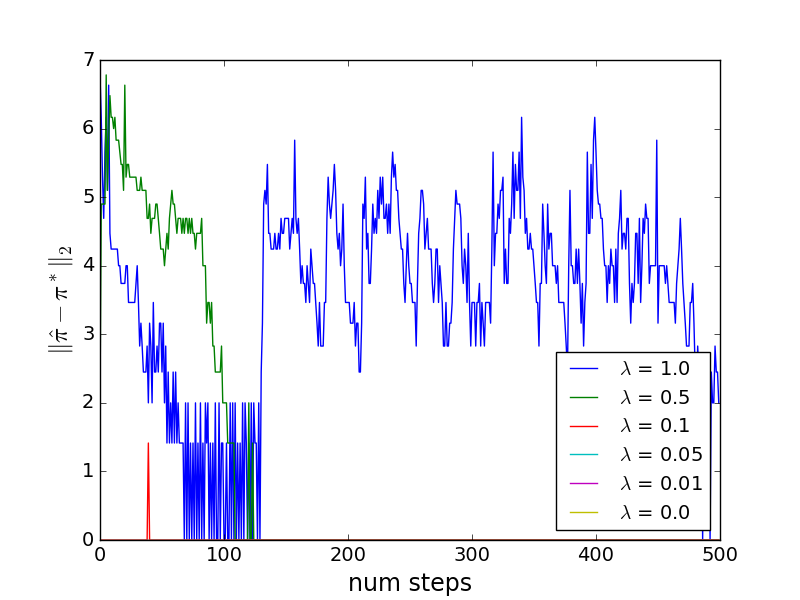
\includegraphics[width=\textwidth]{figs/policy_diff_reg_test.png}
        \caption{Difference between expert policy and learned policy.}
        \label{subfig:reg_policy_diff}
    \end{subfigure}
    \caption{Evaluation of subgradient ascent for different regularization parameters as a function of number of steps.}\label{fig:regularization_test}
\end{figure}

Our results show adding regularization is a way to recover a sparse reward from expert demonstrations. This could be useful in cases where it is known that the domain has only sparse rewards, as well as in general cases as a type of Occam's razor that prefers simpler (sparse) rewards to explain an expert's behavior.
 
\subsection{Stochastic Gradient Descent}
We had initially hoped to use Stochastic Gradient Descent to try to reduce the computation cost of computing the gradient. As derived above, the gradient is of the form 
\begin{eqnarray}
\nabla_R \log P(D | R) = \sum_{(s,a) \in D} \bigg(\alpha \nabla_R Q_R^*(s,a) - \frac{\alpha}{Z_a}\bigg(\sum_{b \in A} e^{\alpha Q_R^*(s,b)} \nabla_R Q_R^*(s,b)\bigg) \bigg).
\end{eqnarray}
At first glance, this appears to be amenable to stochastic gradient descent, since the gradient is a sum of gradients with respect to each state-action pair in the demonstration $D$. However, there is an implicit coupling because of the need to compute the optimal Q-values to compute the gradient for each term in the summation. This requires solving an MDP, which is where the brunt of the computation lies. Thus, if we are going to go through the trouble of calculating the Q-values in order to calculate the gradient with respect to one state-action pair, we should reuse this computation and compute the full gradient rather than repeatedly taking a step for a single state-action pair which would require repeatedly solving for the Q-values after every mini-batch, giving us a noisier gradient step at a nearly identical cost to the full gradient step.


\section{To Do List}
First we need a way to generate navigation tasks. We will develop a simple grid world simulator where there are a finite number of cells on a map that a robot can drive on. Certain cells will contain dangerous terrain that should be avoided and one cell will be the goal location. This domain can easily be scaled up or down as needed by increasing the number of states.

We also need to compute a closed form expression for the gradient of the BIRL likelihood function for performing gradient descent. To compute the gradient we need a way to solve for the optimal policy given a hypothesis reward function. We will implement the policy iteration algorithm to accomplish this task. 

We will then proceed to experiment with different methods for choosing the step size and ways of adding sparsity as mentioned above. 

We will show plots of the error between the learned reward and the true reward as well as the error between the policy performance between the optimal policy and the policy corresponding to the learned reward. We will compare the number of iterations required to achieve low error as well as the computation time needed. Due to the requirement to solve an MDP at every step, it will be important to see which methods can reduce the error in the least amount of gradient steps, thus we hypothesize that BTLS and accelerated methods will improve upon standard gradient descent techniques. Additionally, we hypothesize that adding a regularization term will allow gradient descent to find a better reward function that matches our sparse domain.

\bibliographystyle{plain}
\bibliography{proposal.bib}


\end{document}